\section{A quick overview of the data}

Let's start this tutorial with a quick overview of what the GRAVITY data look like. The document only deal with dual-field data (as opposed to single-field), at the ``astrored'' reduction level (so, not the fully pipeline-reduced ``scivis'' data). There are a couple of important differences between ``astrored'' data and ``scivis'': in the ``astrored'', the DITs are kept separate, whereas to create the ``scivis'', the pipeline average them; and in ``astrored'' files, the phase of the visibility is not corrected for fringe-tracker referencing, dispersion correction, non-common path error correction, etc.). The exoGravity pipeline is based on those dual-field astrored data products.

Two example data file are provided with this tutorial, which correspond to the same exposure made on 51~Eri, during the night of Nov, 11, 2019. The difference between those two files is that one of them contains a few extra corrections data.
\begin{itemize}
\item{Pipeline reduced ``astrored'': \verb|GRAVI.2019-11-11T06:29:03.495_astroreduced.fits|}
\item{With additional info from Sylvestre: \verb|GRAVI.2019-11-11T06:29:03.495_astroreduced_s.fits|}
\end{itemize}

To look at what is inside these data files, you can open one of them files with ``fv''\footnote{https://heasarc.gsfc.nasa.gov/ftools/fv/} (see Figure~\ref{fig:fv})

\begin{figure}
  \begin{center}
    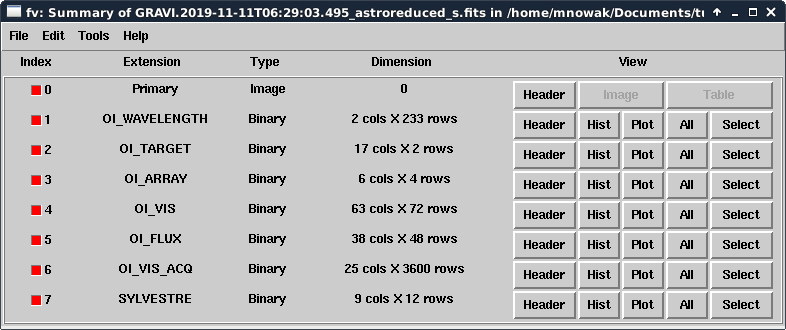
\includegraphics[width=\linewidth]{figures/fv.png}
    \caption{A GRAVITY data file opened with ``fv'', where the different OIs contained in the FITS file are displayed.}
    \label{fig:fv}
  \end{center}
\end{figure}

Each file is divided in different ``OIs'', which contain different fields. Here are the data which are the most useful for exoGravity:
\begin{itemize}
\item{Primary header: The main header contains several useful inforoamtion. Some of the not-so-obvious are: \verb|SOBJ X| and \verb|SOBJ Y|, which give the position of the science fiber with respect to the FT fiber (RA/DEC, in mas); \verb|SOBJ SWAP| tells whether or not the exposure is done at the swapped position; \verb|DET2 SEQ1 DIT| and \verb|NDIT OBJECT| give the integration time (for one DIT, in s), and the number of DITs in the exposure file}
\item{\verb|OI_WAVELENGTH|: \verb|EFF_WAV| contains the wavelength grid, in meters}
\item{\verb|OI_TARGET|: Not used}
\item{\verb|OI_ARRAY|: Not used}
\item{\verb|OI_VIS|: contains the visibiliy (or baseline-based) data. In particular, \verb|VISDATA| contain the complex raw visibilities as extracted by the pipeline, and \verb|VISERR| contain the error on the real and imaginary parts of the \verb|VISDATA|. \verb|UCOORD| and \verb|VCOORD| contain the UV coordinates of the baselines, in meters. \verb|PHASE_REF| contains the phase reference point of the Fringe-Tracker, and \verb|OPD_DISP| contain the OPD dispersion correction}
\item{\verb|OI_FLUX|: contains the flux data, and some important telescope-based quantities related to the metrology correction. \verb|FLUX| and \verb|FLUXERR| give the flux and the associated error bars. The two quantities \verb|OPD_MET_TELFC_MCORR| and \verb|OPD_MET_FC_CORR| are used for the metrology correction (non-common path errors)}
\item{\verb|OI_VIS_ACQ|: Not used}
\item{\verb|SYLVESTRE|: only present in the \verb|_s.fits| file, this extension contains data used for alternative OPD dispersion and metrology corrections}
\end{itemize}



\section{The cleanGravity package}

\subsection{Load a file}

To simplify the manipulation of the data, a dedicated package is provided with the exoGravity pipeline: \verb|cleanGravity|. The aim of that package is to provide an Python object-oriented interface to the GRAVITY data.

Different classes are defined, to fit the specificity of the different GRAVITY file products:
\begin{itemize}
\item{\verb|GravityDualscivisAstrored|}
\item{\verb|GravitySinglefieldsAstrored|}
\item{\verb|GravityDualfieldScivis|}
\item{\verb|GravitySinglefieldScivis|}
\end{itemize}

In the exoGravity pipeline, only \verb|GravityDualfieldAstrored| objects are used. The syntax to load a file into on of these objects is always similar. In the most basic form, you only need to specify the name of the FITS file to load, as well as the extension (when you have different polarizations, you have different extensions): 
\lstinputlisting[linerange={1-3}]{../python/data_manipulation.py}

\noindent{}When the \verb|GravityOi| object is created, several attributes are created:
\begin{itemize}
\item{\verb|oi.header| is an astropy object, which contain the main header}
\item{\verb|oi.visOi| contains the data from the \verb|OI_VIS|. It is a \verb|visOi| object, as defined in the \verb|cleanGravity| package}
\item{\verb|oi.fluxOi| contains the data from the \verb|FLUX_VIS|, in a \verb|fluxOi| object}
\item{Several useful attributes are also loaded from the header, like \verb|oi.sObjX| and \verb|oi.sObjY| (position of the fiber), \verb|oi.mjd| (time of observation), etc. Please refer to the documentation of the package}
\end{itemize}

Once the \verb|GravityOi| object is created, the different data sets are automatically loaded and reshaped in numpy arrays, complex or reals (depending on the data). The shape of these arrays is always:
\begin{equation*}
\text{Shape of the numpy data arrays in cleanGravity:} \qquad \left[n_\mathrm{DIT}, n_\mathrm{channels}, n_\mathrm{wav}\right]
\end{equation*}
\noindent{}Where $n_\mathrm{DIT}$ is the number of DITs in the exposure file, $n_\mathrm{channels}$ the number of channels in the OI (4 channels corresponding to 4 telescopes in the \verb|FLUX_OI|, 6 channels for 6 baselines in \verb|VIS_OI|), and $n_\mathrm{wav}$ corresponds to the number of wavelength points.

\noindent{}For example:
\lstinputlisting[linerange={5-6}]{../python/data_manipulation.py}

\noindent{}As another example, you can plot the flux on each telescope as a function of wavelength using something like:
\lstinputlisting[linerange={8-17}]{../python/data_manipulation.py}

\subsection{Plotting with gravityPlot}

The visibility data contained in \verb|oi.visOi.visData| are complex numbers. To plot them, you need to separate real/imaginary, modulus/phase, or use 3D graphs. To make things easier for a quick view at the data, the \verb|cleanGravity| also provides some plotting functions. These are not automatically loaded at the import of the package, to allow for changing the configuation of \verb|matplotlib| if needed, before importing the plot functions. You can import these functions, and plot the visibilities in real/imaginary parts using:
\lstinputlisting[linerange={19-22}]{../python/data_manipulation.py}

The \verb|modPhasePlot| function does the same thing, but in modulus/phase instead of real/imaginary parts. You can also plot a real quantity over several channels at once using the \verb|baselinePlot| function. For example, instead of looping over the telescopes to plot the flux, you can use the one-liner:
\lstinputlisting[linerange={24-25}]{../python/data_manipulation.py}


\subsection{Standard phase corrections}

The \verb|cleanGravity| package also provides methods to apply the phase corrections to the ``astrored'' data. The FT referencing is automatically applied when the data are loaded, and the resulting ``FT referenced'' visibilities are available in \verb|oi.visOi.visRef|. To apply the OPD dispersion correction, just call \verb|oi.corrDisp()|, or \verb|oi.corrDispSylvestre()|, if you want to use the Sylvestre special correction (only with a \verb|_s.fits| file). Similarly, to apply the metrology (non common path) correction, call \verb|oi.corrMet()|, or \verb|oi.corrMetSylvestre()|.

The phase corrections are always performed on the \verb|oi.visOi.visRef| arrays. The \verb|oi.visOi.visData| stays at the initial values, which give the raw visibilities.

These corrections can be automatically applied when loading the data, by setting the \verb|corrDisp| or \verb|corrMet| kwargs:
\lstinputlisting[linerange={27-28}]{../python/data_manipulation.py}

